\chapter{Discussion}\label{disc}
\thispagestyle{plain}
In this chapter a deeper analysis of the results from chapter \ref{chap3} are presented in order to try to understand the behavior of the models and compare their performances. A comparison of the results obtained with the models used in this thesis to the model presented by \cite{Farinotti2019} will also be presented as it is interesting to compare statistical based models as those deriving from machine learning algorithm to the physical based ones from  \cite{Farinotti2019}.

\section{Machine learning models performances}\label{MLcomp}

One of the easiest approaches to infer the reliability of a model is to check how good is the model at predicting known values. When doing this for a model coming from a machine learning algorithm one needs to be careful at not over-fitting the model, i.e. having a model which is very good at making predictions for data points coming from the data used for training the model but very bad at predicting values for data not used for training. For this reason the models have all been trained using 20 different sub-samples and checking the how good they were doing when making predictions using data left out from the sub-samples used for training.
None of the three models used seem to do a very good job at predicting the ice thickness based on their scores. In the best case in fact the support vector regression had an average score of 0.55 but with a high variance due to sub-samples 5, 14 and 19 having a much lower score. Even the best performing of the trained models which still was one of the support vector regression models trained only had a score just above 0.6. This means that the best model only explain 60\% of the variance of the thickness observations fro the GlaThiDa database.

\begin{figure}[!tp]
	\centering		  
	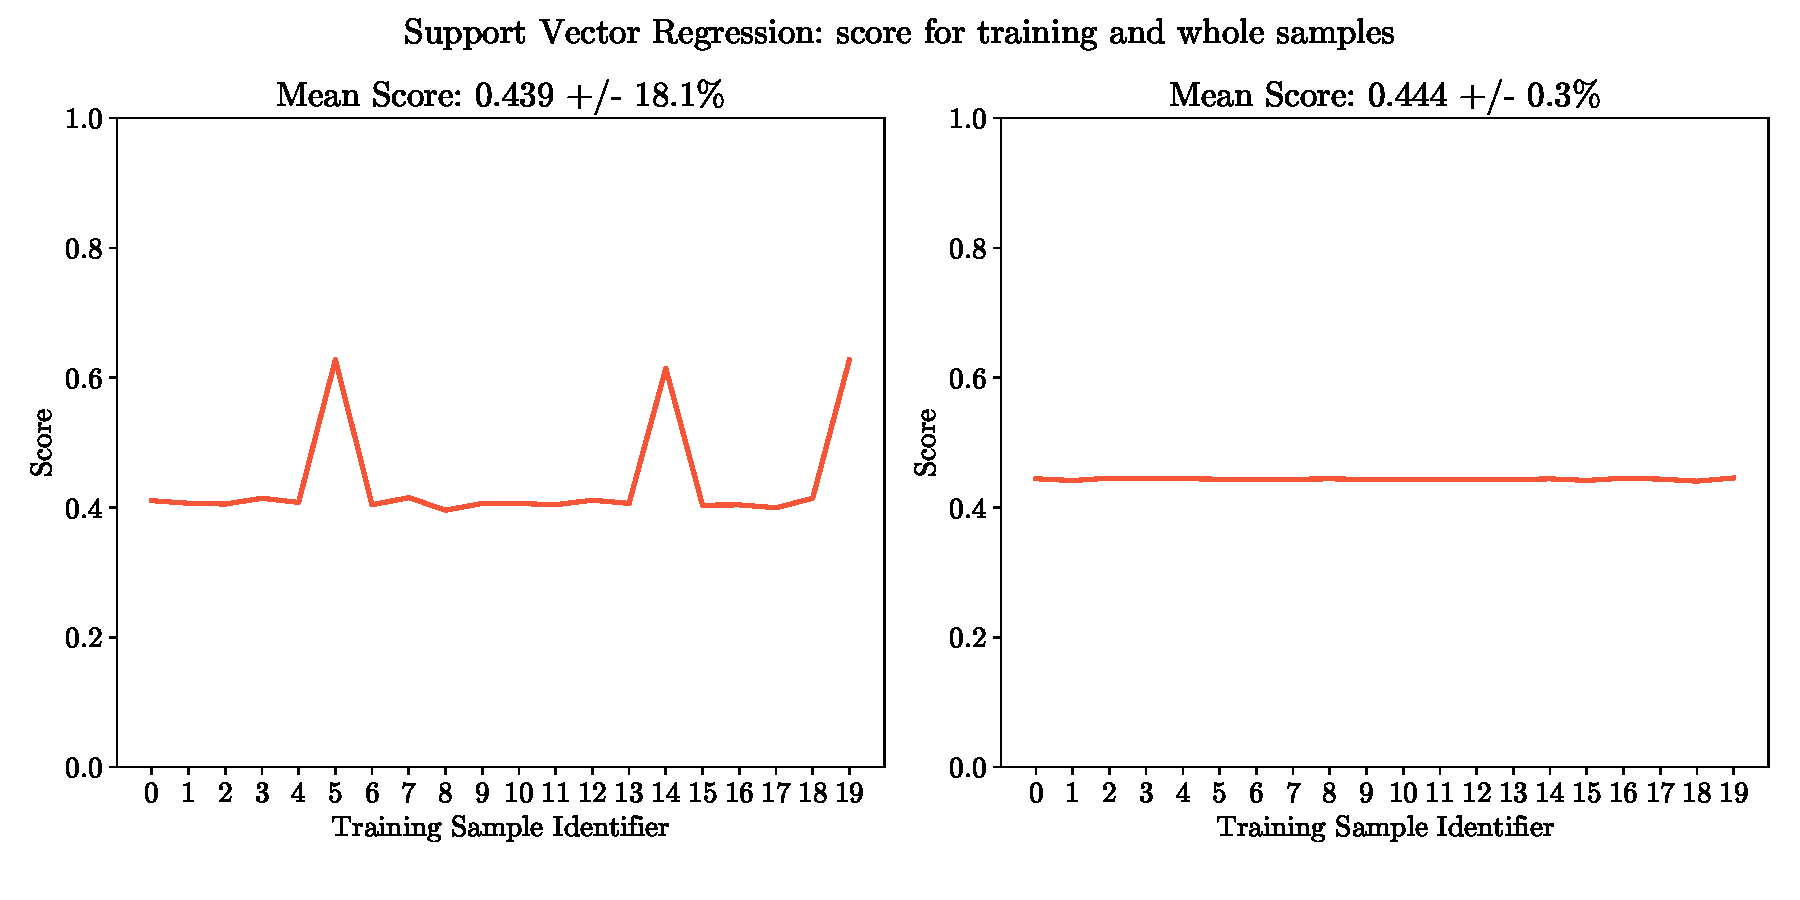
\includegraphics[width=1.\textwidth]{figures/SVR_score_tr.pdf}
	\caption{Support Vector Regression: on the left score achieved by the models trained with the different sub-samples calculated using the training sample instead if the testing sample; on the right the score computed on the whole sub-sample (train and testing data)}
	\label{fig:train-score}
\end{figure}

Interestingly all the models have drop in performance for the sub-samples  5, 14 and 19. A possible explanation of this behavior could be explained by the fact that the sub-sample used for training these models could be missing some data points in the training set which were essential for training a model leading to accurate predictions. If for example those sub-sample had a very different value distribution in any of the attributes used for training compared to the distribution of the whole data-set, it could lead to a biased model not capable of making accurate predictions. This, however difficult to compute exactly, doesn't seem to be the case when looking at Fig. \ref{fig:distribution} showing box-plots of the data distribution for each of the attributes and sample.
Fig. \ref{fig:train-score} shows the score achieved by the support vector machine by the models trained with the different sub-samples. On the right the score was calculated only on the sample used for training in each sub-sample. This in contrast with the results shown in chapter \ref{chap3} which showed the score computed on the data not used for training in each sub-sample. The left chart shows how the highest scores are achieved for sub-samples 5, 14, and 19. Those are the same sub-samples which were showing the lowest scores when computing the score on the testing samples. On the right we can see the scores computed on the whole data-set. The scores are almost constant throughout the sub-samples. All this could be indicating that the reason for the drop in scores showed in chapter \ref{chap3} could be attributed to the fact that the samples left out for testing are particularly difficult to compute for the model. Similar results can be shown also for the linear regression model and for the random forest regression.

\begin{figure}[!tp]
	\centering		  
	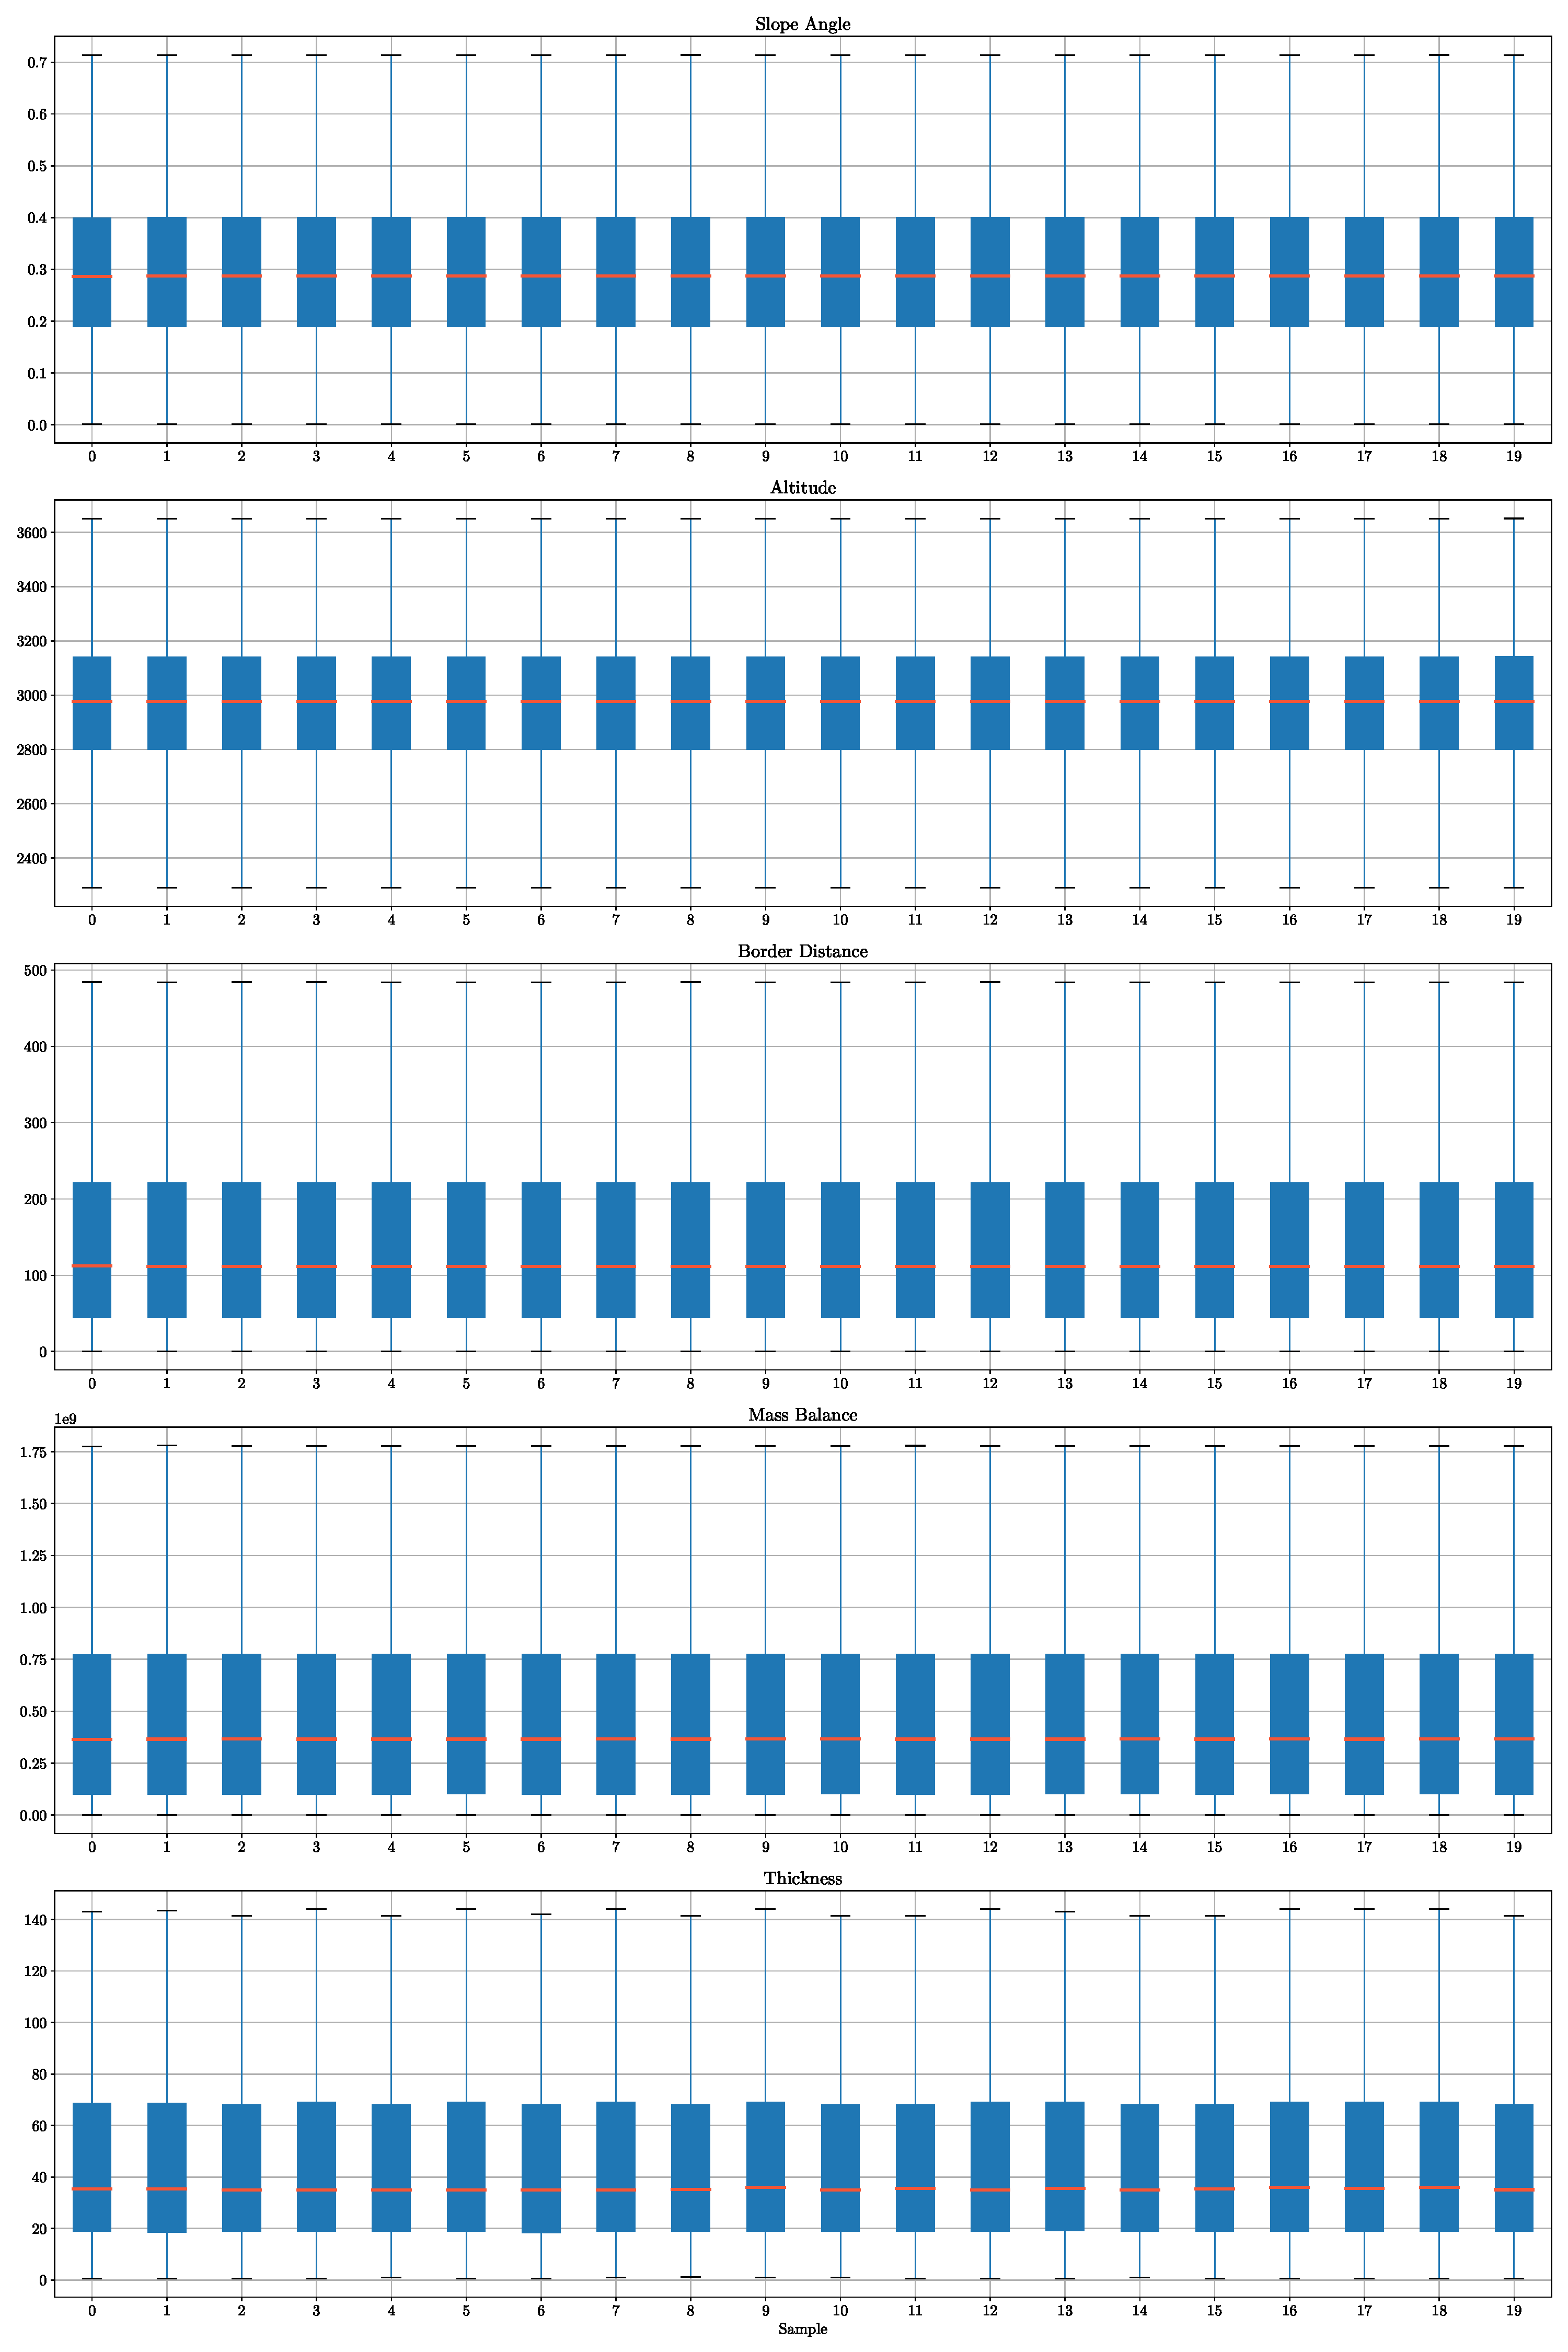
\includegraphics[width=1.\textwidth]{figures/samples_distribution.pdf}
	\caption{Distribution of the attributes used for training the models along the different sub-samples}
	\label{fig:distribution}
\end{figure}

\subsection{Score comparison}
How well do the models predict values in the test dataset and how do the models compare with each other.

\subsection{Spread Comparison}
How much spread can we expect across different slpits between train and test data for all the model.

\subsection{Feature importance comparison}
Do different models give more importance to different features when making predictions?

\section{Alps volume comparison}\label{Alpscomp}
How do the predicted volumes for the whole alps from the machine learning models compare to the volumes predicted by some physical based models.

%The discussion is the interpretation and evaluation of the results. It is a
%comparison of your results with previous findings. It provides the answer to the
%scientific questions raised in the introduction. It is the ``nerve center'' of a
%thesis, whereas the chapter Results may be seen as the ``heart''.
%
%Clearly separate between your own contributions and those of others. Provide
%rigorous citations of appropriate sources! Explicitly refer to specific results
%presented earlier. A certain amount of repetition is necessary. For
%example, the results presented in \ref{3sec:2} suggest that \dots. Order
%discussion items not chronologically but rather logically.
%
%The chapter Results answers the question: \emph{What} has been
%found? (Facts). The chapter Discussion answers the question: \emph{How} has the
%result to be interpreted? (Opinion).
%
%The most important message should appear in the first paragraph. The answer to
%the key question may appear in the first sentence: e.g., did your original idea
%work, or didn't it? The following questions may be answered in the discussion
%section:
%\begin{itemize}
%\item Why is the presented method simpler, better, more reliable than previous
%ones?
%\item What are its strengths and its limitations?
%\item How significant are the results?
%\item How trustworthy are the observations?
%\item Under which precondition/assumption and for which region are the
%results/method valid?
%\item Can the results be easily transferred to other regions or fields?
%\end{itemize}
